\section{Principes de bases des systèmes radar et de l'imagerie SAR}
\subsection{Généralités radar}

Avant d'aborder les techniques avancées d'imagerie SAR, il est nécessaire de rappeler certains concepts fondamentaux des systèmes radar. 

Un système radar émet une onde électromagnétique qui se propage dans l'espace selon la directivité de l'antenne, comme le montrent les traits bleus de la figure \ref{fig:schema_explicatif_radar}. Lorsque cette onde rencontre une cible, des échos sont émis ; ce sont les traits jaunes de la même figure. Ces échos se propagent dans l'espace dans de multiples directions, amplitudes et phases. Ils peuvent également se heurter à d'autres surfaces, générant ainsi de nouveaux échos. Une partie des échos de l'onde incidente est captée par l'antenne du radar et analysée afin d'obtenir plusieurs informations. Il est possible d'extraire la distance relative de la cible à l'antenne, sa vitesse ou encore sa structure \cite{skolnik2001}. 

\begin{figure}[htbp]
    \centering
    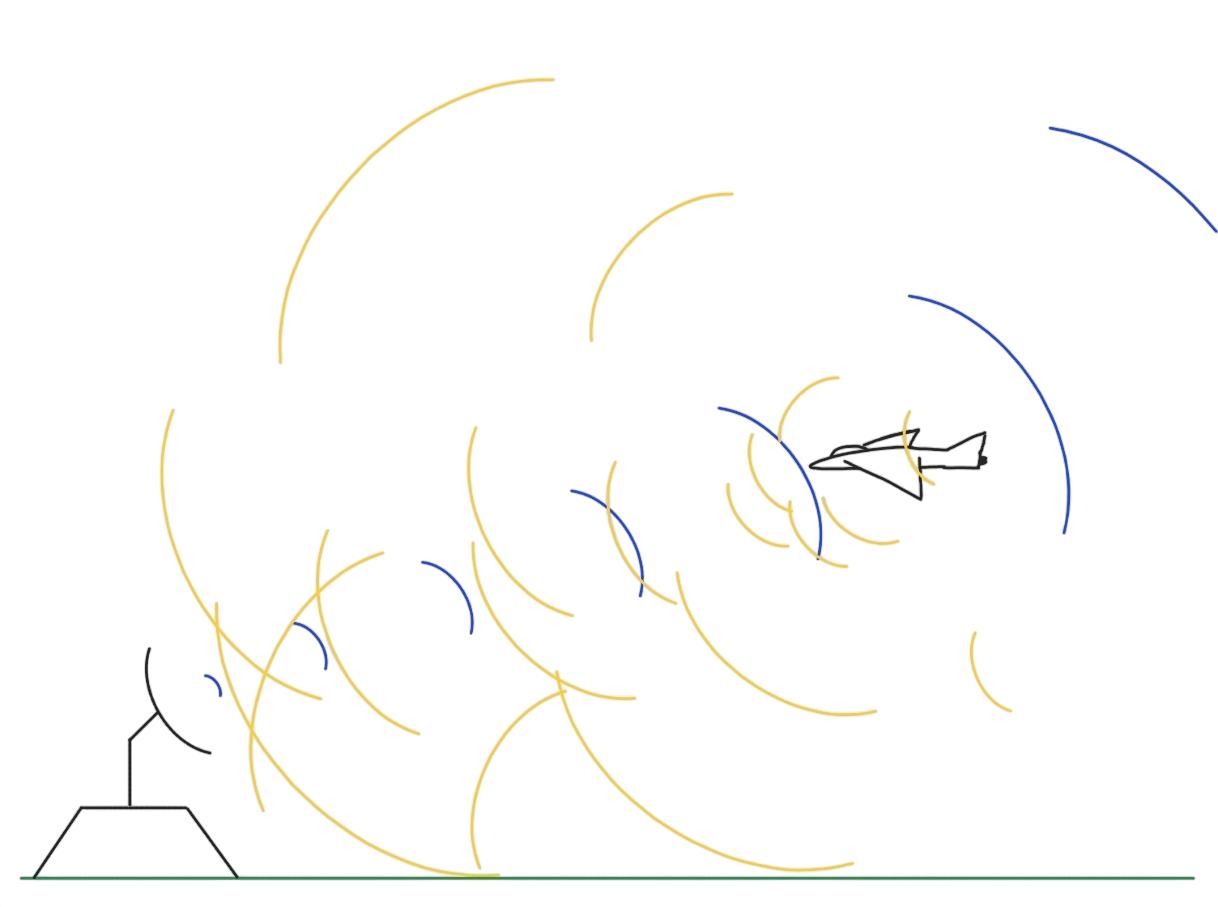
\includegraphics[width=0.5\linewidth]{src/rapport_complet/img/schema_base_radar.png}
    \caption{Schéma d'explication des bases d'un système radar}
    \label{fig:schema_explicatif_radar}
\end{figure}

Il est ensuite possible d'exprimer la puissance reçue par l'antenne par l'équation radar \cite{richards2010} :

\begin{equation}
    P_r \propto \frac{P_t . G^2 . \lambda^2 \sigma}{R^4}
    \label{eq:equation_radar}
\end{equation}
Où : 
\begin{description}
    \item[$P_r$] : est la puissance reçue par l'antenne [$W$]
    \item[$P_t$] : est la puissance transmise par l'antenne [$W$]
    \item[$G$] : est le gain de l'antenne (émission/réception)
    \item[$\lambda$] : est la longueur d’onde [$m$]
    \item[$\sigma$] : est la surface équivalente radar [$m^2$]
    \item[$R$] : est la distance entre l'antenne et la cible [$m$]
\end{description}

L'onde émise l'est selon un angle d'ouverture qui détermine la directivité du faisceau. En clair, un faisceau plus étroit permettra de capter plus d'échos et d'observer plus loin, mais il est nécessaire d'avoir une approximation de la position de la cible. A l'inverse, une antenne peu directive permettra d'observer une zone au détriment de la distance. L'un pourra servir au suivi de la cible, tandis que l'autre permettra de surveiller une zone. L'angle d'ouverture peut être approximé par l'équation suivante :

\begin{equation}
    \theta \approx \frac{\lambda}{L}
    \label{eq:approx_angle_ouverture_antenne}
\end{equation}
Où :
\begin{description}
    \item[$\theta$] : est l'angle d'ouverture [$rad$]
    \item[$\lambda$] : est la longueur d’onde [$m$]
    \item[$L$] : est la longueur physique de l'antenne [$m$]
\end{description}

Afin de déterminer la vitesse de la cible, on utilise l'effet Doppler-Fizeau \cite{skolnik2001}. La figure \ref{fig:illustration_effet_doppler} l'illustre, celui-ci décrit la modification de la fréquence d'une onde observée lorsque la source et/ou l'observateur sont en mouvement relatif. Un rapprochement entre la source et l'observateur entraîne une augmentation de la fréquence perçue tandis qu'un éloignement provoque une diminution de celle-ci. La variation de fréquence correspond à la fréquence Doppler qui s'exprime telle que :

\begin{equation}
    f_d = \frac{2.\nu_r.f_0}{c_0}
    \label{eq:frequence_doppler}
\end{equation}
Où :
\begin{description}
    \item[$f_d$] : est la fréquence Doppler [$Hz$]
    \item[$\nu_r$] : est la vitesse relative à l'émetteur [$m.s^{-1}$]
    \item[$f_0$] : est la fréquence émise [$Hz$] 
    \item[$c_0$] : est la célérité d'une OEM \footnote{Onde Électro-Magnétique} dans le vide [$m.s^{-1}$] 
\end{description}

\begin{figure}[htbp]
    \centering
    \begin{tikzpicture}
    % --- Éléments centraux ---
    \node (radar) at (0,0) {\scalebox{-1}[1]{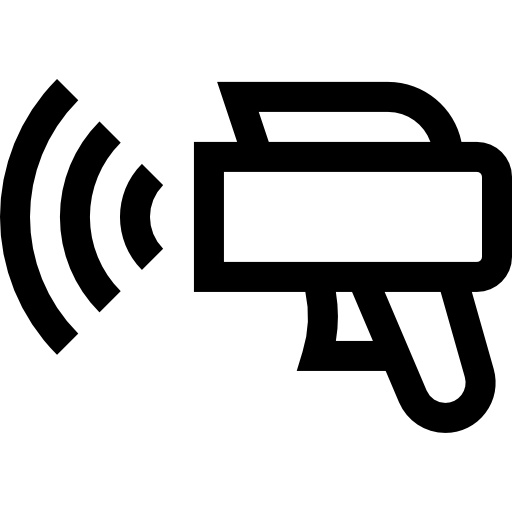
\includegraphics[width=1.5cm]{src/rapport_complet/img/radar-de-vitesse.png}}};
    % domain=1:7 -> dessine de x=1 à x=7
    % 0.2*sin(12*(\x-1.5) r) -> {Amplitude}*sin({Fréquence}*... r)
    \draw[black, thick, smooth] plot[domain=1:7, samples=1000] (\x, {0.4*sin(12*(\x-1.5) r)});
    \draw[-latex, thick] (7.5,0) -- ++(1,0) node[pos=0.5, above] {\(f_o\)};
    % --- Scénario 1 : Le véhicule s'approche ---
    \begin{scope}[yshift=1.5cm]
        % Onde réfléchie (fréquence plus élevée)
        \draw[black, thick, smooth] plot[domain=1:7, samples=1000] (\x, {0.4*sin(24*(\x-1) r)});
        \draw[-latex, thick] (0.5,0) -- ++(-1,0) node[pos=0.5, above] {\(f_o + f_d\)};
        \node (truck_approaching) at (9,0) {\scalebox{-1}[1]{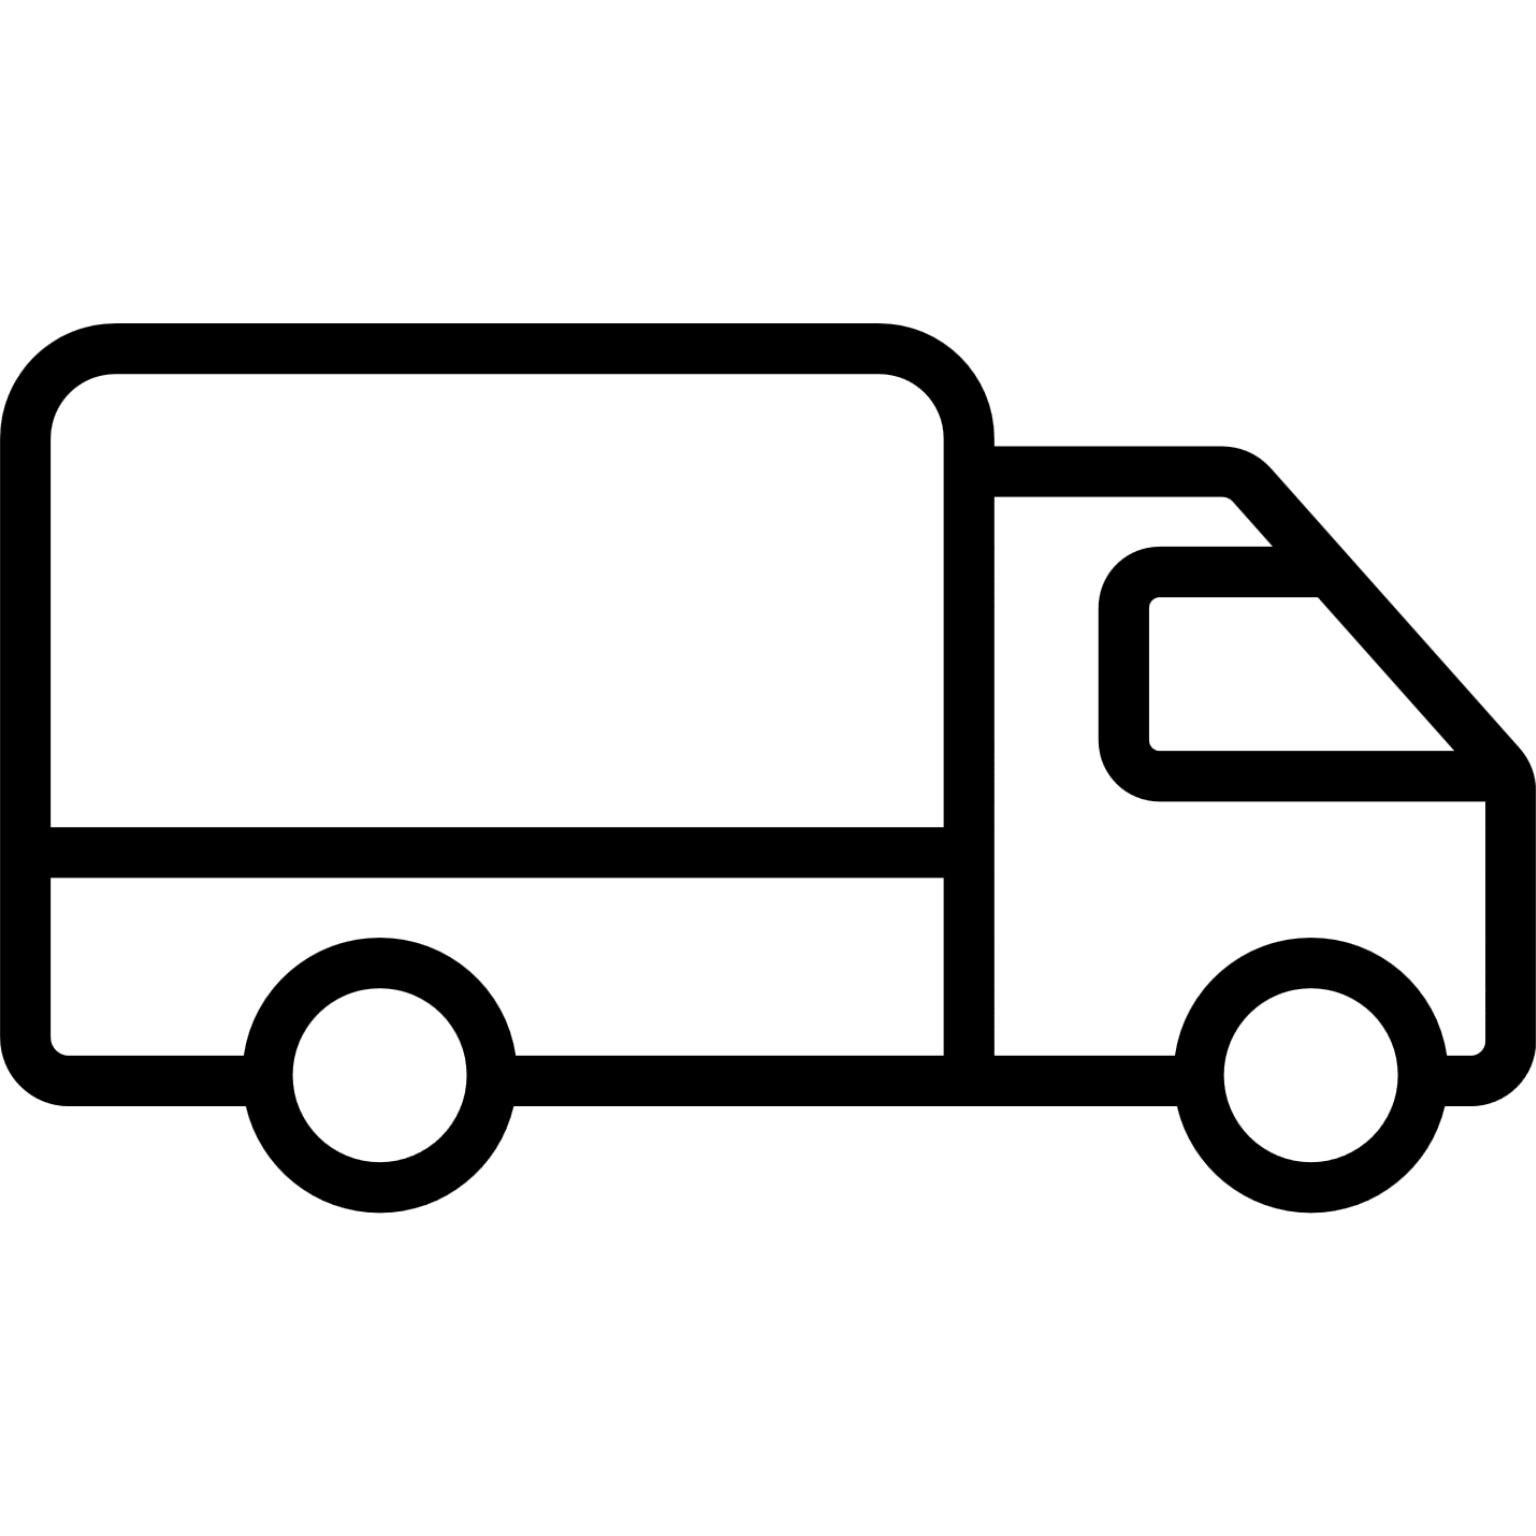
\includegraphics[width=1.5cm]{src/rapport_complet/img/truck-icon.png}}};
        \draw[-latex, thick] (truck_approaching) -- ++(-1.5,0);
    \end{scope}
    % --- Scénario 2 : Le véhicule s'éloigne ---
    \begin{scope}[yshift=-1.5cm]
        \node (truck_receding) at (8.25,0) {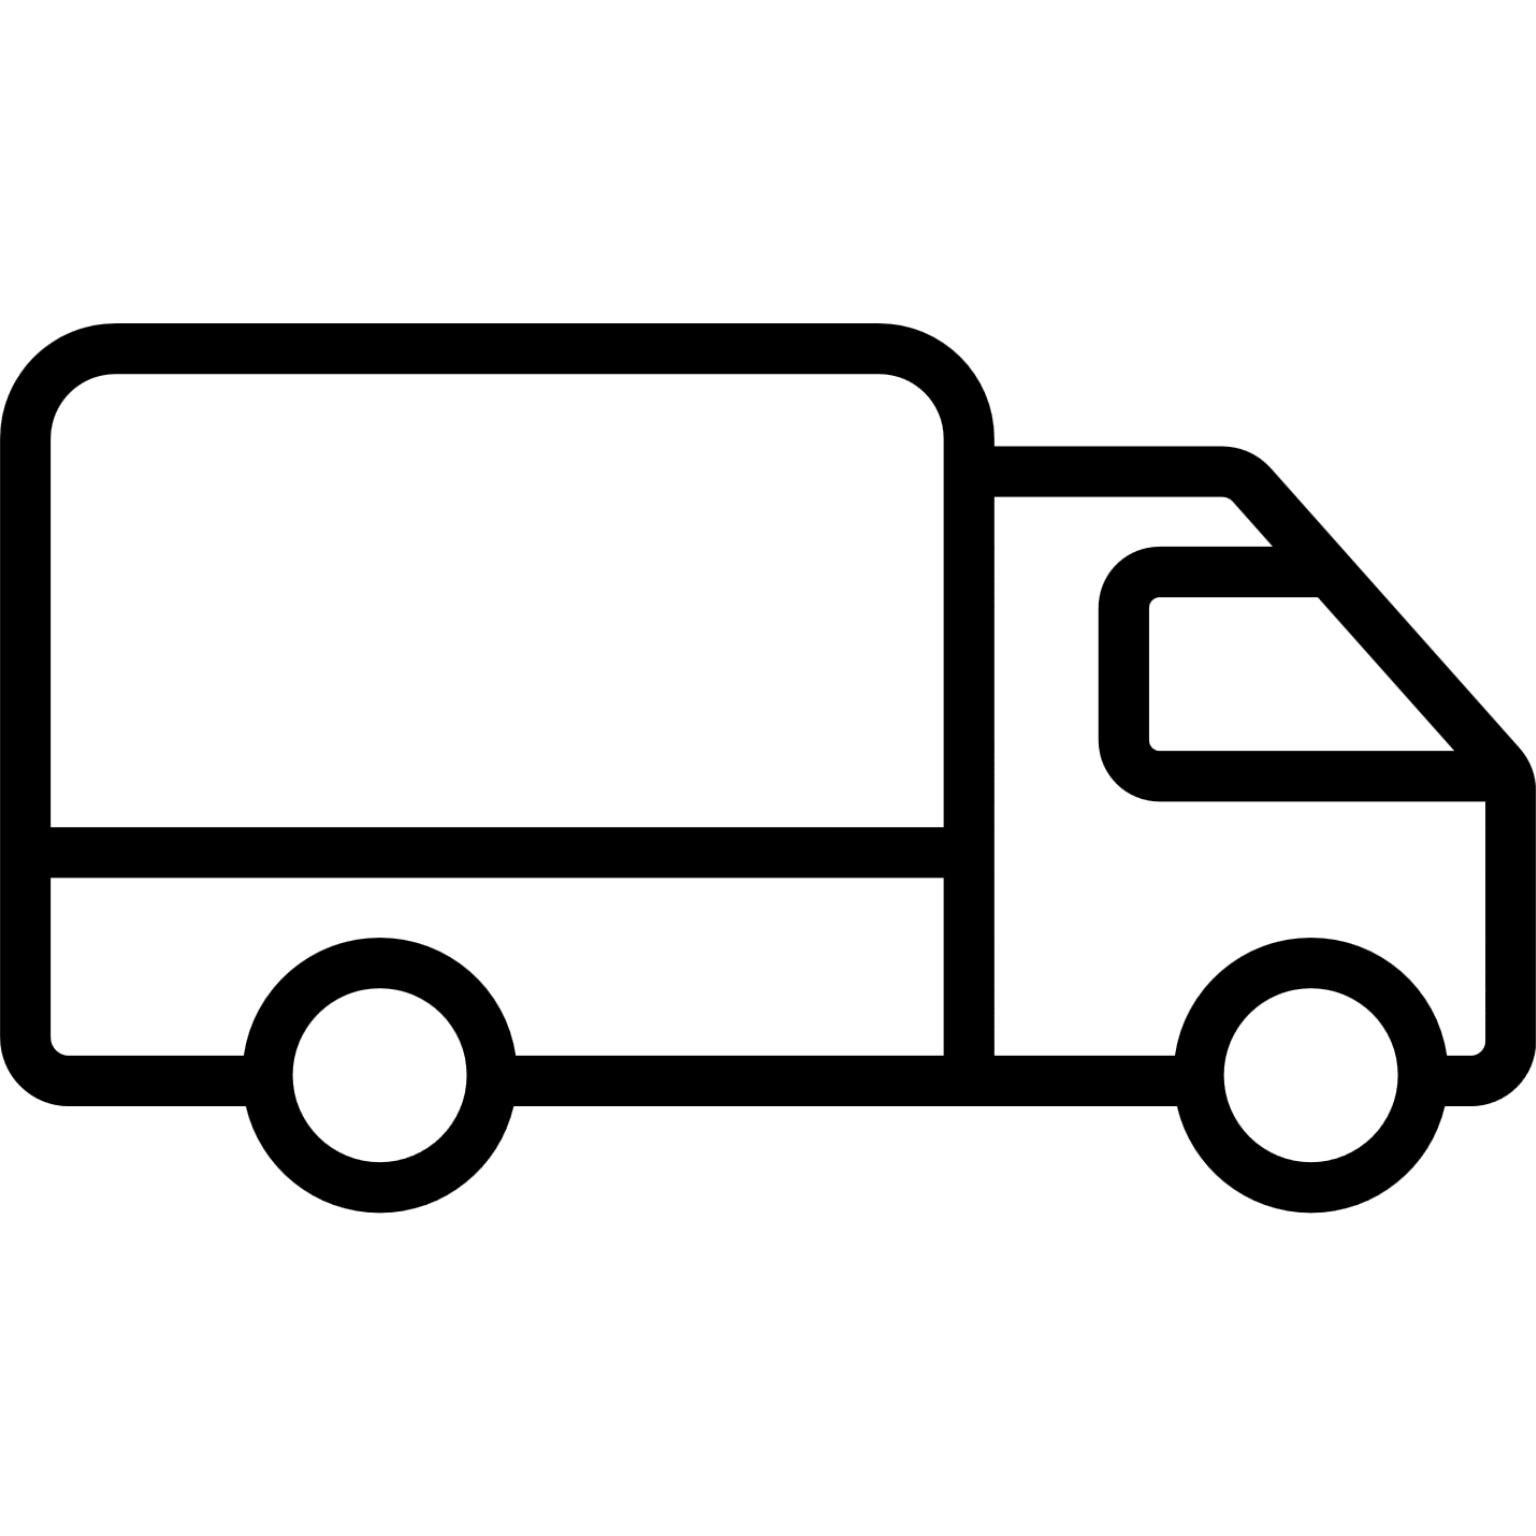
\includegraphics[width=1.5cm]{src/rapport_complet/img/truck-icon.png}};
        \draw[-latex, thick] (truck_receding) -- ++(1.5,0);
        % Onde réfléchie (fréquence plus basse)
        \draw[black, thick, smooth] plot[domain=1:7, samples=1000] (\x, {0.4*sin(6*(\x-1) r)});
        \draw[-latex, thin] (0.5,0) -- ++(-1,0) node[pos=0.5, below] {\(f_o - f_d\)};
    \end{scope}
    \end{tikzpicture}
    \caption{Illustration de l'effet Doppler-Fizeau}
    \label{fig:illustration_effet_doppler}
\end{figure}

\subsection{Formes d'ondes radar}
La performance d’un système radar ne dépend pas uniquement de sa géométrie ou de la puissance transmise, mais également de la nature du signal émis. Le choix de la forme d’onde conditionne à la fois la portée, la résolution et la sensibilité du radar. Selon les applications, différentes formes d’onde sont employées, qu’elles soient continues ou modulées, à impulsions courtes ou à large bande.

Il existe trois catégories de formes d'onde : 
\begin{itemize}
    \item les impulsions simples,
    \item les impulsions modulées,
    \item les ondes continues.
\end{itemize}

\subsubsection{Impulsions simples}
Les impulsions simples, aussi appelées pulse, consistent en l'émission d'une impulsion courtes et puissantes de signal radar. Chaque impulsion est suivie d'une période de silence qui permet au radar d'écouter les échos des cibles, ces mêmes échos qui permettent de déterminer la distance et la vitesse relative de la cible au radar. La figure \ref{fig:impulsions_radar_avec_echo} permet d'illustrer le fonctionnement de cette forme d'onde.

\begin{figure}[htbp]
    \centering
    \begin{tikzpicture}[label/.style={font=\small}]
        % --- Définition des paramètres ---
        \def\periodeTp{7}             % Période de répétition des impulsions (Tp)
        \def\largeurImpulsion{0.3}    % Largeur de l'impulsion (τp)
        \def\retardEcho{4}            % Retard de l'écho (τe)
        \def\amplitudeEmise{3}        % Amplitude de l'impulsion émise
        \def\amplitudeEcho{0.5}       % Amplitude de l'écho
        \def\xstart{1}                % Position de départ pour le dessin
        % --- Dessin des axes ---
        \draw[-{Stealth[length=3mm]}, thick] (-0.5, 0) -- (\xstart+\periodeTp+\largeurImpulsion+1.5, 0) node[below] {$t$};
        \draw[-{Stealth[length=3mm]}, thick] (0, -1) -- (0, \amplitudeEmise+1) node[left] {Amplitude};
        \node[below left] at (0,0) {0};
        % --- Dessin des signaux ---
        % Ligne de base et impulsions émises (noir)
        \draw[thick] (\xstart-1, 0) -- (\xstart, 0)
            -- (\xstart, \amplitudeEmise) -- (\xstart+\largeurImpulsion, \amplitudeEmise) -- (\xstart+\largeurImpulsion, 0) -- (\xstart+\periodeTp, 0) -- (\xstart+\periodeTp, \amplitudeEmise) -- (\xstart+\periodeTp+\largeurImpulsion, \amplitudeEmise) -- (\xstart+\periodeTp+\largeurImpulsion, 0) -- (\xstart+\periodeTp+\largeurImpulsion+1, 0);
        % Impulsion de l'écho (rouge)
        \draw[thick, red] (\xstart+\retardEcho, 0) -- (\xstart+\retardEcho, \amplitudeEcho) -- (\xstart+\retardEcho+\largeurImpulsion, \amplitudeEcho) -- (\xstart+\retardEcho+\largeurImpulsion, 0);
        % --- Annotations ---
        % Annotation de Tp (Période de répétition)
        \draw[dashed, gray] (\xstart, \amplitudeEmise) -- (\xstart, \amplitudeEmise+0.5) -- (\xstart+\periodeTp, \amplitudeEmise+0.5) -- (\xstart+\periodeTp, \amplitudeEmise);
        \node[label, above] at (\xstart+\periodeTp/2, \amplitudeEmise+0.5) {$T_p$};
        % Annotation de τe (Retard de l'écho)
        \draw[dashed, gray] (\xstart+\largeurImpulsion, 0) -- (\xstart+\largeurImpulsion, -0.7) -- (\xstart+\retardEcho, -0.7) -- (\xstart+\retardEcho, 0);
        \node[label, below] at (\xstart+\largeurImpulsion+\retardEcho/2, -0.7) {$\tau_e$};
        % Annotation de τp (Largeur de l'impulsion) - CORRIGÉ
        \draw[dashed, gray] (\xstart, \amplitudeEmise) -- (\xstart, \amplitudeEmise+1) -- (\xstart+\largeurImpulsion, \amplitudeEmise+1) -- (\xstart+\largeurImpulsion, \amplitudeEmise);
        \node[label, above] at (\xstart+\largeurImpulsion/2, \amplitudeEmise+1) {$\tau_p$};
    \end{tikzpicture}
    \caption{Représentation d'impulsions simples avec un écho d'un radar}
    \label{fig:impulsions_radar_avec_echo}
\end{figure}

Les impulsions et l'écho représentés dans la figure \ref{fig:impulsions_radar_avec_echo} correspondent aux périodes où une sinusoïde est émise ou captée. Pour détecter l'écho, le radar va appliquer un filtre adapté au signal reçu. Si le signal reçu comporte un écho, cette opération va faire apparaître un pic de corrélation. Ce dernier permet la mesure de $\tau_e$ qui correspond au temps nécessaire à l'écho pour être capté par le radar. Grâce à cette mesure, on peut calculer la distance relative de la cible au radar. Ce calcul n'est possible que puisque le canal de propagation est connu et constant.

L'utilisation du pic de corrélation pour détecter l'écho implique que si deux cibles sont proches comparés à la durée d'impulsions, elles seront confondues. Ainsi la résolution en distance est exprimée par l'équation suivante \cite{richards2010, radartutorial} :

\begin{equation}
    \delta_d \geq \frac{c_0 . \tau_p}{2} = \frac{c_0}{2. B}
    \label{eq:resolution_distance_pulse}
\end{equation}
Où :
\begin{description}
    \item[$\delta_d$] : est la résolution en distance [$m$]
    \item[$c_0$] : est la célérité d'une OEM dans le vide [$m.s^{-1}$]
    \item[$\tau_p$] : est la durée d'émission d'une impulsion [$s$]
    \item[$B$] : est la bande de fréquence de l'impulsion [$Hz$]
\end{description}

Ainsi, on en déduit que pour obtenir la meilleure résolution en distance, il faut émettre une impulsion plus fine. Cependant, cette forme d'onde possède une ambiguïté concernant la distance 

Une autre problématique de cette forme d'onde est l'ambiguïté concernant la distance relative de la cible au radar. En effet, un écho résultant d'une impulsion peut être détecté après l'impulsion suivante. Ainsi, il n'est pas possible de déterminer la distance de la cible, la portée maximale non ambiguë d'un radar à impulsion s'exprime de la manière suivante \cite{skolnik2001,radartutorial} : 

\begin{equation}
    \delta_{max} = \frac{c_0 . (T_p - \tau_p)}{2}
    \label{eq:resolution_distance_max_radar_pulse}
\end{equation}
Où :
\begin{description}
    \item[$\delta_{max}$] : est la portée maximale non ambiguë [$m$]
    \item[$c_0$] : est la célérité d'une OEM dans le vide [$m.s^{-1}$]
    \item[$T_p$] : est le temps de répétition des impulsions [$s$]
    \item[$\tau_p$] : est la durée d'émission d'une impulsion [$s$]
\end{description}

Cette forme d'onde permet aussi d'évaluer la vitesse de la cible grâce à l'effet Doppler-Fizeau. Cependant, la résolution en vitesse s'exprime telle que : 

\begin{equation}
    \delta\nu_r = \frac{\Delta f_d.\lambda_0}{2} = \frac{\lambda_0}{2.\tau_p} = \frac{\lambda_0.B}{2}
    \label{eq:resolution_vitesse_impulsions}
\end{equation}
Où :
\begin{description}
    \item[$\delta\nu_r$] : est la résolution en vitesse [$m.s^{-1}$]
    \item[$\Delta f_d$] : est la différence entre les deux fréquences Doppler [$Hz$] 
    \item[$\lambda_0$] : est la longueur d'onde de la fréquence émise [$m$] 
    \item[$\tau_p$] : est la durée d'impulsion [$s$]
    \item[$B$] : est la bande de fréquence de l'impulsion [$Hz$]
\end{description}

On remarque que pour obtenir une bonne résolution en vitesse, il faut une durée d'impulsion $\tau_p$ très grande. Or, c'est l'exact opposé du critère permettant l'obtention d'une bonne résolution en distance. Il faut donc réaliser un compromis entre les deux critères ou bien utiliser d'autres formes d'ondes \cite{richards2010}. 

Les radars pulsés sont généralement utilisés pour de la surveillance aérienne, les relevés météorologiques et les systèmes de navigations.

\subsubsection{Impulsions modulées}
La forme d'onde FMCW \footnote{Frequency Modulated Continuous Wave} Sawtooth utilise une modulation en dents de scie, aussi appelées "chirp", où la fréquence augmente et diminue de manière répétée comme l'illustre la figure \ref{fig:impulsions_chirp_avec_echo}. Elle permet de mesurer la distance et la vitesse mais il y a une ambiguïté entre les deux termes \cite{cumming2005}.

\begin{figure}[htbp]
    \centering
    \begin{tikzpicture}[
        label/.style={font=\small, black},
        annotation/.style={black, thick},
        axis/.style={thick, gray!50!black}, % Couleur pour les axes
        gridline/.style={dashed, gray} % Style pour les lignes de grille/verticales
    ]
        % --- Définition des paramètres ---
        \def\Ts{3}       % Période de la rampe (T_s)
        \def\Bch{2.5}    % Bande passante / Amplitude (B_ch)
        \def\retard{0.6} % Retard temporel (\tau_e)
        \def\nramps{3}   % Nombre de rampes à dessiner
        % --- Dessin des axes ---
        % Axe horizontal (temps)
        \draw[-{Stealth[length=3mm]}, axis] (-0.5,0) -- (\nramps*\Ts + \Ts + 1,0) node[right,black] {$t$};
        % Axe vertical (fréquence)
        \draw[-{Stealth[length=3mm]}, axis] (0,-0.5) -- (0,\Bch + 0.8) node[above,black] {$f(t)$};
        \node[below left, black] at (0,0) {0};
        % --- Dessin des signaux et lignes verticales ---
        \foreach \i in {0,...,\nramps} {
            % Signal transmis (noir) - en dents de scie
            \draw[black, thick] (\i*\Ts, 0) -- (\i*\Ts + \Ts, \Bch);
            % Lignes verticales pour le signal noir
            \ifnum\i<\nramps % Ne pas dessiner la dernière ligne verticale si elle sort du graphique
                \draw[black, thick] (\i*\Ts + \Ts, 0) -- (\i*\Ts + \Ts, \Bch);
            \fi
        }
        \foreach \i in {0,...,\nramps} {
            % Signal écho (rouge) - retardé dans le temps
            \draw[red, thick] (\i*\Ts + \retard, 0) -- (\i*\Ts + \Ts + \retard, \Bch);
             % Lignes verticales pour le signal rouge
             % On peut ajouter une condition si on ne veut pas qu'elles s'étendent trop loin
             \ifnum\i<\nramps % Ne pas dessiner la dernière ligne verticale si elle sort du graphique
                 \draw[red, thick] (\i*\Ts + \Ts + \retard, 0) -- (\i*\Ts + \Ts + \retard, \Bch);
             \fi
        }
        % --- Annotations ---
        % Annotation \tau_e (Retard temporel)
        \draw[<->, annotation] (0, -0.3) -- (\retard, -0.3) node[midway, below, label] {$\tau_e$};
        % Annotation T_s (Période)
        % On la place au-dessus, entre le début de la 2ème et 3ème rampe
        \draw[<->, annotation] (\Ts, \Bch+0.3) -- (2*\Ts, \Bch+0.3) node[midway, above, label] {$T_s$};
        % Annotation B_ch (Bande passante)
        % On la place à droite pour correspondre à l'image
        \draw[<->, annotation] (-0.25, 0) -- (-0.25, \Bch) node[midway, left, label] {$B_{ch}$};
        % Annotation \Delta f = f_b (Fréquence de battement)
        % On choisit un point dans le temps pour montrer la différence de fréquence
        % Positionnée au milieu de la 3ème rampe noire
        \def\annotXpos{2*\Ts + 0.5*\Ts} 
        % Coordonnée sur le signal noir à x = \annotXpos
        % La rampe n°2 (i=2) va de x=2*Ts à 3*Ts. L'équation est y = (Bch/Ts) * (x - 2*Ts)
        \coordinate (point_noir) at (\annotXpos, {(\Bch/\Ts) * (\annotXpos - 2*\Ts)});
        % Coordonnée sur le signal rouge à x = \annotXpos
        % L'écho de la rampe n°2 va de x=2*Ts+retard à 3*Ts+retard. L'équation est y = (Bch/\Ts) * (x - retard - 2*\Ts)
        \coordinate (point_rouge) at (\annotXpos, {(\Bch/\Ts) * (\annotXpos - \retard - 2*\Ts)});
        \draw[<->, annotation] (point_rouge) -- (point_noir) node[midway, below right, label] {$\Delta f = f_b$};
    \end{tikzpicture}
    \caption{Représentation d'une impulsion Chirp et de son écho}
    \label{fig:impulsions_chirp_avec_echo}
\end{figure}

Comme pour les impulsions, la détection de l'écho s'effectue avec un filtre adapté. Cependant la résolution en distance n'est plus la même. En effet, la modulation Sawtooth modifie la fréquence sur la bande $B_{ch}$ ce qui permet d'avoir un pic de corrélation plus marqué et donc plus simple à détecter même lorsque deux cibles sont proches. La résolution est alors \cite{cumming2005} : 

\begin{equation}
    \delta_d = \frac{c_0}{2.B_{ch}}
    \label{eq:resolution_en_distance_chirp}
\end{equation}
Où :
\begin{description}
    \item[$\delta_d$] : est la résolution en distance [$m$]
    \item[$c_0$] : est la célérité d'une OEM dans le vide [$m.s^{-1}$]
    \item[$B_{ch}$] : est la bande des fréquences modulées du chirp [$Hz$]
\end{description}

On remarque alors que plus la bande de fréquence du chirp est grande, meilleure est la résolution (i.e. plus faible). De plus, pour mesurer une vitesse grâce à une OEM, on utilise l'effet Doppler-Fizeau qui modifie la fréquence en fonction de la vitesse comme explicité par l'équation (\ref{eq:frequence_doppler}). Or dans le cas de la modulation Sawtooth, on utilise la modulation de fréquence pour émettre notre signal. Ainsi, la modification de la fréquence due à la vitesse change la corrélation entre le filtre adapté et le signal reçu, ce qui apporte une ambiguïté entre la distance et la vitesse.

Cette forme d'onde est par exemple utilisé dans des radar de surveillance maritime ou des applications industrielles.

Il existe une autre forme d'onde qui permet de résoudre ces limitations : la FMCW triangulaire. Illustrée par la figure \ref{fig:fmcw_avec_echo}, elle consiste en l'émission d'un chirp montant et descendant. On peut alors déterminer sans ambiguïté la distance et la vitesse en résolvant le système de fréquences de battement mesurées sur les deux rampes \cite{richards2010}.

\begin{figure}[htbp]
    \centering
    \begin{tikzpicture}[label/.style={font=\small}]
        % --- Définition des paramètres ---
        \def\Tr{5}      % Période de la rampe (T_r)
        \def\Amp{2.5}    % Amplitude (correspond à B_ch / 2)
        \def\retard{0.8} % Retard temporel (\tau_e)
        \def\doppler{0.3} % Décalage en fréquence (f_d)
        % --- Dessin des axes ---
        \draw[-{Stealth[length=3mm]}, thick] (-0.5,0) -- (2.2*\Tr,0) node[right] {$t$};
        \draw[-{Stealth[length=3mm]}, thick] (0,-0.5) -- (0,\Amp+1) node[above] {$f(t)$};
        \node[below left] at (0,0) {0};
        % --- Signal transmis (en bleu) ---
        \draw[black, thick] (0,0) -- (\Tr/2, \Amp) -- (\Tr, 0) -- (1.5*\Tr, \Amp) -- (2*\Tr, 0);
        % --- Signal reçu (en rouge) ---
        \draw[red, thick] (\retard, \doppler) -- (\Tr/2+\retard, \Amp+\doppler) -- (\Tr+\retard, \doppler) -- (1.5*\Tr+\retard, \Amp+\doppler) -- (2*\Tr+\retard, \doppler);
        % --- Annotations et lignes de repère ---
        % Lignes pointillées et ticks sur l'axe des temps (VERSION SIMPLIFIÉE)
        \foreach \pos/\labeltext in {\retard/\tau_e, \Tr/T_r} {\draw[dashed, gray] (\pos, -0.1) -- (\pos,0);\node[below, label] at (\pos, -0.1) {$\labeltext$};}
        % Annotation de B_ch
        \draw[<->, thick] (-0.3, 0) -- (-0.3, \Amp) node[midway, left, label] {$B_{ch}$};
        % --- Annotation du retard (\tau) ---
        % Lignes pointillées partant du sommet de chaque signal
        \draw[dashed, gray] (\Tr/2, \Amp) -- (\Tr/2, \Amp+1); % Ligne du pic bleu
        \draw[dashed, gray] (\Tr/2+\retard, \Amp+\doppler) -- (\Tr/2+\retard, \Amp+1); % Ligne du pic rouge
        % Ligne horizontale supérieure et le label
        \draw[dashed, gray] (\Tr/2, \Amp+1) -- (\Tr/2+\retard, \Amp+1);
        \node[above, label] at (\Tr/2+\retard/2, \Amp+1) {$\tau_e$};
        % --- Annotation de f_d ---
        \def\fdXpos{\Tr/2+\retard+1} % Position en x de la flèche f_d (décalée de 1)
        % Ligne pointillée du pic bleu jusqu'à la flèche f_d
        \draw[dashed, gray] (\Tr/2, \Amp) -- (\fdXpos, \Amp);
        % Ligne pointillée du pic rouge jusqu'à la flèche f_d
        \draw[dashed, gray] (\Tr/2+\retard, \Amp+\doppler) -- (\fdXpos, \Amp+\doppler);
        % La flèche f_d, décalée vers la droite
        \draw[<->] (\fdXpos, \Amp) -- (\fdXpos, \Amp+\doppler) node[midway, right, label] {$f_d$};
        % Annotation des fréquences de battement (fb_up et fb_dw)
        % f_b^up
        \def\upPos{1.5} % Position en x pour l'annotation
        \coordinate (A) at (\upPos, {(\Amp/(\Tr/2))*(\upPos - \retard) + \doppler});
        \coordinate (B) at (\upPos, {(\Amp/(\Tr/2))*\upPos});
        \draw[<->, thick] (A) -- (B) node[midway, below right, label] {$f_b^{up}$};
        % f_b^dw
        \def\dwPos{4} % Position en x pour l'annotation
        \coordinate (C) at (\dwPos, {\Amp+\doppler - (\Amp/(\Tr/2))*(\dwPos - \Tr/2 - \retard)});
        \coordinate (D) at (\dwPos, {\Amp - (\Amp/(\Tr/2))*(\dwPos - \Tr/2)});
        \draw[<->, thick] (C) -- (D) node[midway, below right, label] {$f_b^{dw}$};
    \end{tikzpicture}
    \caption{Représentation de la forme d'onde FMCW et d'un écho}
    \label{fig:fmcw_avec_echo}
\end{figure}

La résolution en distance peut alors s'exprimer de la manière suivante :

\begin{equation}
    \delta_d = \frac{c_0}{2.B_{ch}}
    \label{eq:resolution_distance_fmcw_triangulaire}
\end{equation}
Où :
\begin{description}
    \item[$\delta_d$] : est la résolution en distance [$m$]
    \item[$c_0$] : est la vitesse d'une OEM dans le vide [$m.s^{-1}$]
    \item[$B_{ch}$] : est la bande des fréquences modulées [$Hz$]
\end{description}

Et la résolution en vitesse :

\begin{equation}
    \delta\nu_r = \frac{c_0}{2.f_0.T_r}
    \label{eq:resolution_vitesse_fmcw_triangulaire}
\end{equation}
Où :
\begin{description}
    \item[$\delta\nu_r$] : est la résolution en vitesse [$m.s^{-1}$]
    \item[$c_0$] : est la vitesse d'une OEM dans le vide [$m.s^{-1}$]
    \item[$f_0$] : est la fréquence centrale [$Hz$]
    \item[$T_r$] : est la période du signal [$s$]
\end{description}

On remarque ainsi que les deux résolutions ne sont pas inversement liées. On peut donc avoir une bonne résolution en distance et une bonne résolution en vitesse. Cependant, cet avantage doit être nuancé par la complexité de la réalisation matérielle de cette forme d'onde, d'autant plus sur une large bande. 

Cette forme d'onde est généralement utilisée par des radars de contrôle de la circulation, systèmes de détection de collision et les capteurs de distance.

\subsection{Rapport signal sur bruit}
Toutes les figures et équations présentées précédemment représentent la vision théorique et sans bruit des formes d'onde. Or, dans un  système réel, le signal est perturbé par différentes sources de bruit, cette perturbation est exprimée par le rapport signal sur bruit.

[TODO] equation SNR, modélisation stochastique du bruit, limites, impact sur le traitement radar.



BASES SAR ALEXIS : 

\section{Principe du radar SAR}\label{SEC:Principe du radar SAR}

\subsection{Rappel du principe SAR}

Synthèse d’ouverture par le déplacement du radar.

Notions de bande azimutale, résolution, longueur d’onde, vitesse de plateforme.


\subsection{Types de SAR}

Le choix de la forme d’onde constitue un paramètre fondamental dans la conception d’un radar à synthèse d’ouverture (SAR), notamment lorsqu’il est embarqué sur une plateforme légère telle qu’un drone. Chaque forme d’onde possède des caractéristiques spécifiques qui influencent directement les performances en portée, en résolution, en complexité électronique et en robustesse face au bruit ou aux interférences \cite{richards2010principles, soumekh1999synthetic}.

La forme d’onde impulsionnelle (Pulse) représente historiquement le schéma le plus simple. Elle consiste à émettre des impulsions brèves et puissantes séparées par des intervalles de silence. Ce mode offre une bonne résolution en distance si la largeur d’impulsion est courte, mais impose une puissance crête élevée, difficile à générer sur des plateformes à ressources énergétiques limitées comme les drones. De plus, l’efficacité énergétique du radar impulsionnel est faible, car l’émetteur reste inactif une grande partie du temps. Ainsi, bien que cette forme d’onde soit robuste et bien maîtrisée, elle est souvent peu adaptée aux systèmes SAR compacts embarqués sur UAV \cite{skolnik2008radar}.

Les formes d’onde FMCW (Frequency Modulated Continuous Wave), en particulier les modulations en dent de scie et triangulaire, offrent une alternative attractive. Dans le cas du FMCW en dent de scie, la fréquence du signal augmente linéairement au cours du temps avant de revenir instantanément à sa valeur initiale. Ce type de modulation permet de mesurer la distance et la vitesse de la cible à partir du décalage de fréquence entre le signal émis et reçu. Son avantage principal réside dans la faible puissance crête requise et la simplicité de l’électronique d’émission \cite{ma2016compact}. Cependant, la récupération simultanée des informations de portée et de vitesse peut devenir complexe en présence de cibles multiples, et la discontinuité de la rampe peut introduire des artefacts dans le traitement SAR.

Le FMCW triangulaire, quant à lui, alterne des montées et descentes de fréquence successives, ce qui permet une mesure plus précise de la vitesse radiale (via la différence de battement entre les deux pentes). Cette propriété réduit l’ambiguïté Doppler et améliore la qualité des images SAR, en particulier lorsque la plateforme est en mouvement continu, comme c’est le cas pour un drone \cite{meta2007performance}. Toutefois, cette forme d’onde nécessite un étalonnage précis du temps de montée et de descente, ainsi qu’une correction fine des non-linéarités de la modulation pour éviter la dégradation de la résolution \cite{aoki2020chirp}.

Enfin, la modulation FSK (Frequency Shift Keying) repose sur une émission séquentielle de fréquences discrètes. Chaque palier correspond à une fréquence fixe pendant un court intervalle de temps. L’avantage majeur de cette approche est la simplicité du traitement de détection, ainsi que la résistance accrue au bruit et aux interférences \cite{li2018fsk}. Néanmoins, la résolution en distance est généralement inférieure à celle des modulations chirpées, et la reconstruction d’image SAR nécessite une interpolation fine des sauts fréquentiels.

Dans le contexte d’un SAR embarqué sur drone, les compromis principaux concernent la consommation énergétique, la résolution en distance et en azimut, et la stabilité fréquentielle de l’émetteur. Les formes d’onde FMCW, en particulier la triangulaire, apparaissent comme un choix privilégié dans la littérature récente pour les radars embarqués légers, grâce à leur efficacité en puissance et à leur compatibilité avec des émetteurs à onde continue de faible coût. Toutefois, des études expérimentales montrent que la correction des distorsions de la rampe de fréquence demeure un défi pour garantir la qualité radiométrique et géométrique des images SAR \cite{sun2021fmcw, yang2023uavsar}.




% Voir si les figures sont cohérentes en rapport avec celles de Maxence
\begin{figure}[ht]
  \centering
  % --- Figure 1 : Pulse ---
  \setlength{\unitlength}{1cm}
  \begin{picture}(10,2)
    \thicklines
    \put(0,0){\line(1,0){0.25}}
    \put(0.25,0){\line(0,2){2}}
    \put(0.25,2){\line(2,0){0.5}}
    \put(0.75,2){\line(0,-2){2}}
    \put(0.75,0){\line(1,0){2.5}}
    \put(3.25,0){\line(0,2){2}}
    \put(3.25,2){\line(2,0){0.5}}
    \put(3.75,2){\line(0,-2){2}}
    \put(3.75,0){\line(1,0){2.5}}
    \put(6.25,0){\line(0,2){2}}
    \put(6.25,2){\line(2,0){0.5}}
    \put(6.75,2){\line(0,-2){2}}
    \put(6.75,0){\line(1,0){2.5}}
    \put(9.25,0){\line(0,2){2}}
    \put(9.25,2){\line(2,0){0.5}}
    \put(9.75,2){\line(0,-2){2}}
    \put(9.75,0){\line(1,0){0.25}}
  \end{picture}
  \caption*{(a) Pulse}

  \vspace{1.5cm} % espace vertical entre les figures

  % --- Figure 2 : Sawtooth FMCW ---
  \setlength{\unitlength}{1cm}
  \begin{picture}(10,2)
    \thicklines
    \put(0,0){\line(1,1){2}}  
    \put(2,2){\line(0,-2){2}}  
    \put(2,0){\line(1,1){2}}
    \put(4,2){\line(0,-2){2}}
    \put(4,0){\line(1,1){2}}
    \put(6,2){\line(0,-2){2}}
    \put(6,0){\line(1,1){2}}
    \put(8,2){\line(0,-2){2}}
    \put(8,0){\line(1,1){2}}
    \put(10,2){\line(0,-2){2}}
  \end{picture}
  \caption*{(b) Sawtooth FMCW}

  \vspace{1.5cm}

  % --- Figure 3 : Triangular FMCW ---
  \setlength{\unitlength}{1cm}
  \begin{picture}(10,2)
    \thicklines
    \put(0,0){\line(1,1){2}}  
    \put(2,2){\line(1,-1){2}} 
    \put(4,0){\line(1,1){2}}
    \put(6,2){\line(1,-1){2}}
    \put(8,0){\line(1,1){2}}
  \end{picture}
  \caption*{(c) Triangular FMCW}

  \vspace{1.5cm}

  % --- Figure 4 : FSK ---
  \setlength{\unitlength}{1cm}
  \begin{picture}(8,3.8)
    \thicklines
    \put(0,1){\line(1,0){1.5}}
    \put(1.5,1){\line(0,1){0.7}}
    \put(1.5,1.7){\line(1,0){1.5}}
    \put(3,1.7){\line(0,1){0.7}}
    \put(3,2.4){\line(1,0){1.5}}
    \put(4.5,2.4){\line(0,1){0.7}}
    \put(4.5,3.1){\line(1,0){1.5}}
    \put(6,3.1){\line(0,1){0.7}}
    \put(6,3.8){\line(1,0){1}}
    \put(7,3.8){\line(0,-1){2.8}}
    \put(7,1){\line(1,0){1}}
  \end{picture}
  \caption*{(d) FSK}

  \caption{Allure des formes d'ondes : (a) Pulse, (b) Sawtooth FMCW, (c) Triangular FMCW, (d) FSK.}
  \label{fig:radar_waveforms}
\end{figure}


% CHECK TABLEAU
\begin{table}[ht]
\centering
\begin{tabular}{|>{\centering\arraybackslash}p{2.75cm}|>{\centering\arraybackslash}p{2.75cm}|>{\centering\arraybackslash}p{2.75cm}|>{\centering\arraybackslash}p{2.75cm}|>{\centering\arraybackslash}p{2.75cm}|}\hline
\textbf{Type de radar} & \textbf{Résolution de la distance} & \textbf{Résolution de la vitesse relative} & \textbf{Avantages} & \textbf{Inconvénients} \\
\hline
\textbf{Pulse} & Haute (dépend de la largeur d'impulsion)  
$\Delta R = \frac{c T_p}{2}$  & Faible (dépend de la fréquence d'échantillonnage)
\par $\Delta v_r = \frac{\lambda_0}{2T_p}$ & Simple à mettre en œuvre, bonne portée & Sensible aux interférences, nécessite un traitement complexe pour la vitesse \\
\hline
\textbf{Sawtooth FMCW} & Modérée (dépend de la pente de la rampe)
$\Delta R = \frac{c}{2 B_{ch}}$ & Modérée (dépend de la fréquence de répétition) 
$\Delta v_r = \frac{c}{2 T_r}$ & Peut mesurer la distance et la vitesse simultanément, mais ambiguïté & Moins efficace que le triangular FMCW pour la vitesse\\
\hline
\textbf{Triangular FMCW} & Très haute (dépend de la largeur de bande)
$\Delta R = \frac{c}{2 B_{ch}}$ & Très haute (peut mesurer des vitesses relatives avec précision) 
$\Delta v_r = \frac{c}{2 T_r}$ & Excellente résolution de distance et de vitesse & Complexité de mise en œuvre, coût plus élevé, résolution entre multiples cibles \\
\hline
\textbf{FSK} & Bonne (dépend du saut de fréquence)
$\Delta R = \frac{c}{2 B_{ch}}$ & Bonne (dépend du temps d'intégration)
$\Delta v_r = \frac{c}{2 T_{obs}}$ & Simple traitement du signal, faible sensibilité au bruit & Résolution moindre que FMCW, complexité pour cibles multiples \\
\hline
\end{tabular}
\caption{Tableau comparatif des formes d'ondes}
\end{table}


\subsection{Contraintes liées à la plateforme drone}

Mouvements instables, vibrations, trajectoire non rectiligne.

Gestion du temps et synchronisation (INS/GNSS, compensation de mouvement).


\subsection{Performances visées}

Résolution en distance et azimut.

Portée, rapport signal/bruit, dynamique.


[TODO] : DEGAGER LA BIBLIO DANS BIBLIOGRAPHY.BIB

\bigskip
\noindent\textbf{Références bibliographiques simulées :}
\begin{thebibliography}{9}
\bibitem{richards2010principles} M. A. Richards, \textit{Principles of Modern Radar: Basic Principles}, SciTech, 2010.
\bibitem{soumekh1999synthetic} M. Soumekh, \textit{Synthetic Aperture Radar Signal Processing}, Wiley, 1999.
\bibitem{skolnik2008radar} M. I. Skolnik, \textit{Radar Handbook}, 3rd ed., McGraw-Hill, 2008.
\bibitem{ma2016compact} J. Ma et al., “Compact FMCW SAR for UAV-based remote sensing,” \textit{IEEE Trans. Geosci. Remote Sens.}, vol. 54, no. 12, 2016.
\bibitem{meta2007performance} A. Meta et al., “Performance analysis of FMCW SAR,” \textit{IEEE Trans. Geosci. Remote Sens.}, vol. 45, no. 11, 2007.
\bibitem{aoki2020chirp} T. Aoki and Y. Sugimoto, “Chirp linearization in low-cost FMCW radar,” \textit{IEEE Sensors Journal}, vol. 20, no. 22, 2020.
\bibitem{li2018fsk} W. Li et al., “FSK-based radar waveform for low-power SAR systems,” \textit{Electronics Letters}, vol. 54, no. 10, 2018.
\bibitem{sun2021fmcw} Y. Sun et al., “FMCW SAR imaging on UAV platforms: System design and calibration,” \textit{Remote Sensing}, vol. 13, no. 3, 2021.
\bibitem{yang2023uavsar} L. Yang et al., “Recent advances in lightweight UAV SAR systems,” \textit{IEEE Aerospace and Electronic Systems Magazine}, vol. 38, no. 1, 2023.
\end{thebibliography}




\newpage


%lié imagerie
Résolution range/radial :

Que veut dire le B ? Le bruit ? 

\begin{equation}
    \delta_{range} \approx \frac{c}{2B}
\end{equation}
Où :
\begin{description}
    \item[$\delta_{range}$] : est la résolution en range [$m$]
    \item[$\lambda$] : est la longueur d’onde [$m$]
    \item[$L$] : est la taille physique de l'antenne [$m$]
\end{description}

Résolution en azimut/latérale :

\begin{equation}
    \delta_{az} \approx \frac{R. \lambda}{L}
\end{equation}
Où :
\begin{description}
    \item[$\delta_{az}$] : est la résolution azimutale [$m$]
    \item[$R$] : est la distance entre l'antenne et la cible [$m$]
    \item[$\lambda$] : est la longueur d’onde [$m$]
    \item[$L$] : est la taille physique de l'antenne [$m$]
\end{description}

Résolution Approximée car la résolution n'est pas la même partout sur la fauchée/tache au sol.

radar cw,
impulsion
chirp
doppler
fmcw
radar pulsé (impulsion ???)

\subsection{Limites des radars conventionnels pour l'imagerie}

\subsection{Principe du SAR}

Plan : 2. Des radars conventionnels à la synthèse d’ouverture
2.1 Rappels fondamentaux sur le fonctionnement radar

(Section de mise en contexte technique avant d’aborder les limites des radars à ouverture réelle.)

2.1.1 Principe général et équation radar

Fonctionnement de base : émission d’une onde électromagnétique, réflexion par la cible, réception de l’écho.

Équation radar simplifiée reliant la puissance reçue à la portée, la puissance émise, le gain d’antenne et la section efficace radar (RCS).

Définition du rapport signal/bruit (SNR) et de son rôle dans la détection.

2.1.2 Portée et sensibilité

Définition de la portée maximale détectable.

Facteurs déterminants : puissance, gains, pertes, bruit de réception.

Compromis entre portée, résolution et temps d’intégration.

2.1.3 Effet Doppler et mesure de vitesse

Rappel du décalage Doppler dû à la composante radiale de la vitesse.

Utilisation du Doppler pour la discrimination de cibles mobiles et pour la mesure de vitesse.

Introduction du lien entre vitesse relative et résolution azimutale dans les systèmes d’imagerie.

2.1.4 Résolution spatiale du radar

Définition de la résolution en distance, dépendant de la bande passante du signal émis.

Définition de la résolution en azimut, dépendant de la largeur du faisceau d’antenne.

Expression de la résolution en azimut d’un radar à ouverture réelle :

%δaz≈λRL
%δ
%az
%	​

%≈
%L
%λR
%	​


où 
%λ
%λ est la longueur d’onde, 
R
R la distance à la cible et 
L
L la longueur physique de l’antenne.

Discussion de la dépendance forte de la résolution à la distance pour les radars à antenne réelle.

2.2 Limites des radars conventionnels pour l’imagerie

(Transition naturelle vers la justification du SAR.)

2.2.1 Contraintes de résolution et dimensionnement d’antenne

Pour obtenir une résolution fine, il faudrait une antenne très longue : contrainte matérielle majeure pour les systèmes embarqués.

Difficulté de maintenir une résolution constante avec la distance (élargissement du faisceau).

2.2.2 Contraintes géométriques et dynamiques

Effets du mouvement de la plateforme sur la stabilité de l’image (flou, désalignement).

Sensibilité aux variations de trajectoire et à la géométrie side-looking typique des radars d’imagerie.

2.2.3 Bruit de speckle (chatoiement)

Définition du speckle comme phénomène d’interférence cohérente entre échos élémentaires.

Nature multiplicative du bruit, affectant le contraste et la lisibilité des images radar.

Origine statistique : fluctuations dues à la cohérence du signal.

Conséquences : difficulté d’interprétation visuelle, nécessité de traitements de réduction (moyennage multilook, filtrage adaptatif, etc.).

2.3 Principe du radar à synthèse d’ouverture (SAR)

(Introduction du SAR comme solution directe aux limites précédemment identifiées.)

2.3.1 Concept général et ouverture synthétique

Idée clé : recréer une grande antenne virtuelle en exploitant le mouvement du radar.

Acquisition successive d’échos cohérents le long de la trajectoire, permettant une ouverture synthétique.

Amélioration drastique de la résolution azimutale, indépendante de la distance à la cible.

2.3.2 Compression en distance et en azimut

Compression en distance : utilisation de signaux modulés en fréquence (chirp) pour obtenir une haute résolution sans sacrifier la portée.

Compression en azimut : traitement Doppler cohérent des signaux successifs pour focaliser l’image en direction transversale.

Étapes clés : formation du signal brut, filtrage de mise en phase, focalisation en azimut.

2.3.3 Résultats et avantages du SAR

Résolution constante et élevée, même à grande distance.

Intégration cohérente du signal → amélioration du SNR.

Production d’images bidimensionnelles précises et exploitables.

2.4 Transition vers les techniques avancées

(Préparer la suite de ta revue bibliographique.)

Le SAR constitue la base des techniques d’imagerie radar modernes (InSAR, PolSAR, TomoSAR…).

Ces variantes exploitent les propriétés de cohérence, polarisation et phase du signal SAR pour étendre les capacités d’analyse.

Rappels radar : portée, Doppler, résolution, SNR.

Limites des radars conventionnels pour l’imagerie.
speckle (chatoiement) 

Principe du SAR : ouverture synthétique, compression en distance et en azimut.




\newpage
1. Introduction

Contexte général : radar, observation tout temps, intérêt civil et militaire.

Besoin d’imagerie haute résolution → limites des radars conventionnels → motivation du SAR.

Positionnement spécifique : SAR embarqué sur drones, multi-capteurs, fusion et détection.

2. Principes de base du radar et du SAR

Rappels radar : portée, Doppler, résolution, SNR.

Limites des radars conventionnels pour l’imagerie.
speckle (chatoiement) 

Principe du SAR : ouverture synthétique, compression en distance et en azimut.

3. Algorithmes de traitement SAR (formation d’image)
3.1 Compression en distance et en azimut
3.2 Algorithmes classiques

Range-Doppler

Chirp Scaling

omega–k (Range Migration Algorithm)

Backprojection

3.3 Limitations et hypothèses

Trajectoire rectiligne idéale, scène plane, hypothèse cible ponctuelle.

Contraintes en bande, navigation et coût calcul.

3.4 Comparaison des algorithmes
4. Avancées récentes en traitement SAR

Compensation de mouvement (MOCO), autofocus.

Traitements temps-fréquence et robustes.

Implémentations temps réel (GPU, FPGA).

Approches émergentes (IA, deep learning pour focalisation).

5. SAR embarqué sur drones (UAV-SAR)
5.1 Intérêt et spécificités

Portabilité, observation basse altitude, flexibilité.

5.2 Contraintes UAV

Masse/énergie, vibrations, trajectoire non idéale, volume de données.

5.3 Travaux académiques (ex. Pelle 2020, projets universitaires)
5.4 Développements industriels (mini-SAR sur drones militaires et civils)
5.5 Algorithmes adaptés

Backprojection robuste, navigation assistée GNSS/IMU, correction post-traitement.

6. Fusion multi-drones et SAR collaboratif
6.1 Intérêt : couverture étendue, redondance, meilleure résolution.
6.2 Contraintes : synchronisation temporelle, cohérence de phase, calibration inter-capteurs.
6.3 Travaux existants : MIMO-SAR, expériences UAV multi-capteurs.
6.4 Limites actuelles et défis pour l’avenir.
7. Détection en imagerie SAR
7.1 Objectif et enjeux de la détection

Cibles ponctuelles vs étendues, clutter, hétérogénéité du milieu.

7.2 Algorithmes classiques de détection

CFAR (CA-CFAR, OS-CFAR, GO-CFAR, SO-CFAR).

Détection par seuillage global et adaptatif.

7.3 Limites des méthodes classiques

Environnements hétérogènes, forte densité de clutter, faible SNR.

7.4 Approches avancées

Détection bayésienne et probabiliste.

Exploitation de l’information polarimétrique/interférométrique.

Apprentissage automatique (SVM, réseaux de neurones).

Deep learning pour la détection et classification d’objets dans les images SAR.

7.5 Évaluation des performances

Probabilité de détection (Pd), taux de fausses alarmes (Pfa).

Jeux de données et benchmarks (MSTAR, OpenSAR, etc.).

8. Discussion et perspectives

Comparaison des approches (formation image vs exploitation).

Verrous scientifiques actuels : navigation précise, traitement distribué, robustesse en clutter.

Perspectives : SAR multi-drones collaboratifs, IA pour fusion + détection en temps réel.

9. Conclusion

Synthèse des connaissances actuelles.

Positionnement de ton projet par rapport à l’état de l’art.





